%!TEX root = ../../diachron-D5_2.tex

\subsection{The User Interface}
\label{sec:UI} 
In the following section, we will describe a set of mockups which will be implemented as a Web User Interface (UI) for the software prototype for assessment and ranking of datasets.
The User Interface will be made up of 3 parts: Details, Statistics and Assessment.
The Quality Framework Web-UI will be a mix of PHP and JavaScript and is envisioned to run on top of OntoWiki, a wiki based on semantic technologies.
The current technologies and extensions available in OntoWiki allow us to reach both the main objectives in this deliverable, and eventually to commence our initial prototypes of the quality framework (e.g. as an enterprise add-on tool to linked data publishers).
Further investigation upon the usability of OntoWiki is still necessary in order to discover if the mentioned application can fulfil further the quality framework's ambitions, beyond the initial prototypes.
The CubeViz extension is used to visualise statistical graphs about the quality metadata of the datasets.
The UI will communicate with the core assessment framework (cf. Figure~\todo{CL: broken reference}\ref{fig:qualityFramework}) via the defined RESTful APIs (cf. Section~\ref{sec:RestAPI}).

\subsubsection{Details Tab}
The Details Tab (Figure~\ref{fig:uiDetailsTab}) will contain the ranked datasets according to a chosen metric by the user from the facet section. 
This is very similar to the datahub.io\footnote{\url{http://www.datahub.io}} interface. 
The user will also be able to enable filters to the datasets, and also to search through the resultant datasets. 
This tab will only display those datasets which have a corresponding Quality Graph, in order to enable the ranking and retrieval of datasets based on quality criteria.

The Details Tab will have the following functionality:
\begin{description}
\item [1. Facets –]
When the datasets are retrieved, a SPARQL query is performed to get all available quality categories used. 
The result set is used to populate the Category box in the facet. 
Once a category is chosen, the dimension box is populated dynamically via a SPARQL query which fetches the dimensions related to the chosen category. 
A similar procedure is done to populate the metric box. 
When a metric is chosen, then the datasets are ranked in ascending order on the right hand side of the container.\todo{CL: The UI should also display the metric value (or some stars)}
\item [2. Filters –]
Filters will dynamically change according to the chosen metric. 
That is, if the \texttt{daq:expectedDatatype} (cf. Section~\ref{sec:DAQ}) of a metric is boolean then we have a filter which can be a true/false checkbox, whilst if we have a metric with a double type then we could have some slider regulating the minimum value for the metric.
\item [3. Buttons –]
The buttons have the same functionality as in CKAN. 
The additional button \emph{quality metadata/$\langle$file type$\rangle$} returns the quality graph in a specific format. 
The \emph{Visualise Quality} button takes the user to the Statistics tab in the web page.
\end{description}

\begin{figure*}[tbph]
\center
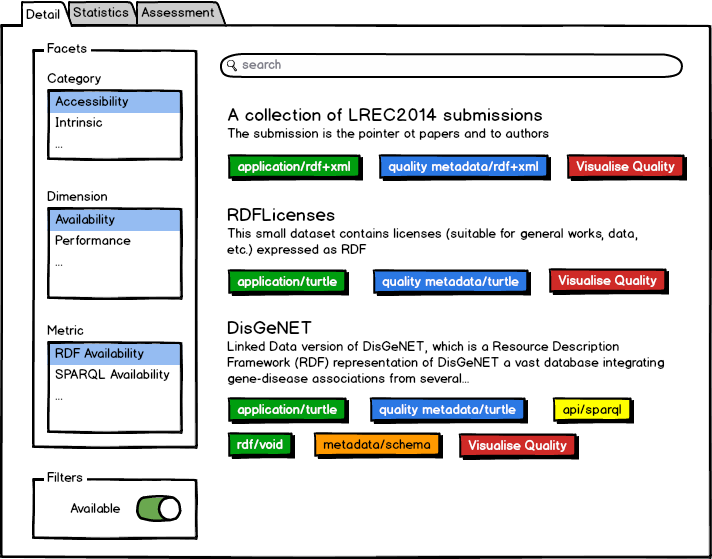
\includegraphics[width=\textwidth]{images/uiDetailsTab.png} 
\caption{Mockup for the Details Tab} 
\label{fig:uiDetailsTab}
\end{figure*}

\subsubsection{Statistics Tab}
The Quality Assessment Framework Web-UI will also give the opportunity to its users to visualise statistical information about a dataset quality.
The Statistical Tab (Figure~\ref{fig:uiStatisticsTab}) will present the user with a number of graphs (cf. Visualisation Layer - Figure~\ref{fig:qualityFramwork} for the description of the different visualisation graphs).
Users can compare different datasets together or even how a dataset changed in its quality over time.

\begin{figure*}[tbph]
\center
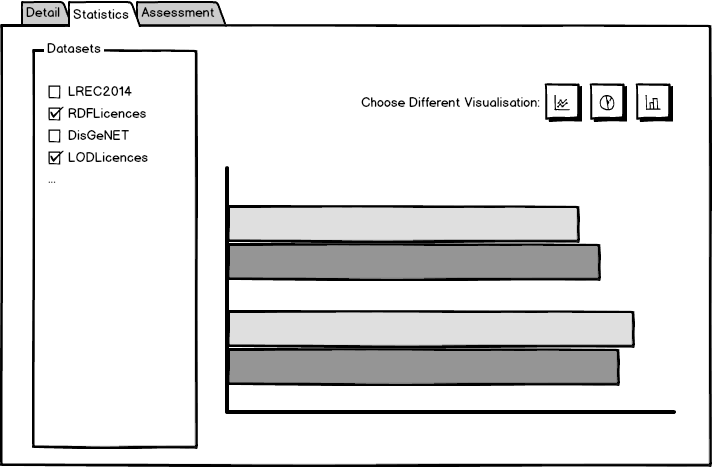
\includegraphics[width=\textwidth]{images/uiStatisticsTab.png} 
\caption{Mockup for the Statistics Tab} 
\label{fig:uiStatisticsTab}
\end{figure*}

\subsubsection{Visualisation Layer}
\label{sec:vislayer_hla}
CubeViz is an extension of the OntoWiki\footnote{\url{http://ontowiki.eu/Welcome}} data wiki for visualising data cubes (observation instances).
Figures~\ref{fig:hor_chart},~\ref{fig:ver_chart},~\ref{fig:rad_chart}, and~\ref{fig:line_chart} depicts four different CubeViz chart visualisations from computed quality metadata\footnote{The quality metadata used can be found in \url{https://raw.githubusercontent.com/diachron/quality/master/src/test/resources/cube_qg.trig}}.  While these are generic chart types, we briefly discuss their specific suitability for data quality analysis.

\begin{figure*}[tbph]
\center
  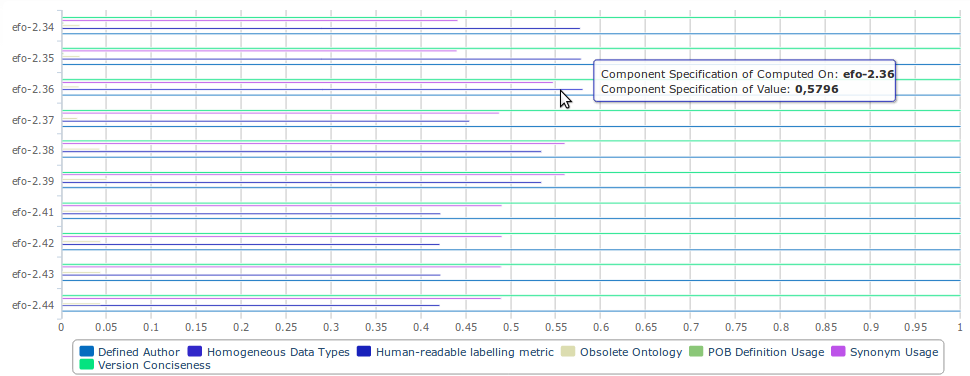
\includegraphics[scale=0.3]{images/cube_1.png}
\caption{Horizontal Bar Chart} 
  \label{fig:hor_chart}
\end{figure*}

\begin{figure*}[tbph]
\center
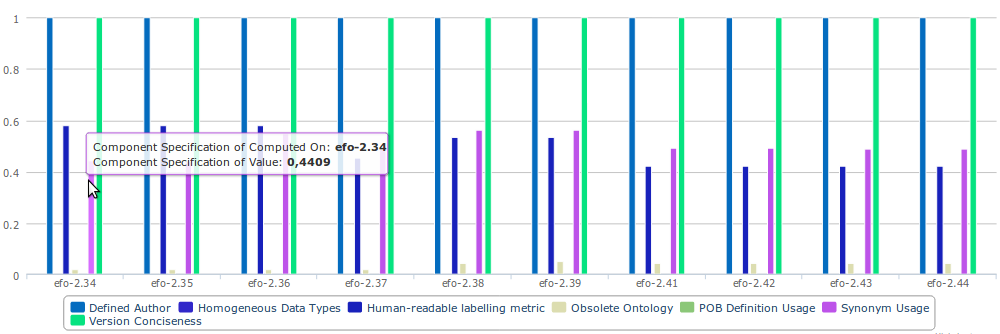
\includegraphics[scale=0.3]{images/cube_2.png} 
\caption{Vertical Bar Chart} 
\label{fig:ver_chart}
\end{figure*}

\begin{figure*}[tbph]
\center
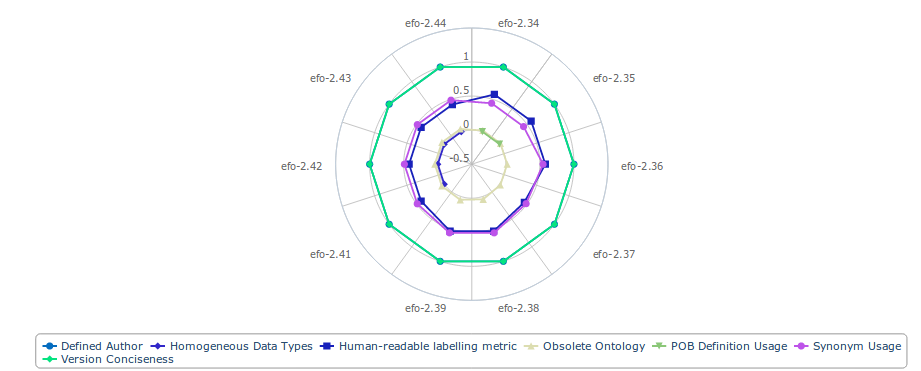
\includegraphics[scale=0.3]{images/cube_3.png} 
\caption{Radar Chart} 
\label{fig:rad_chart}
\end{figure*}

\begin{figure*}[tbph]
\center
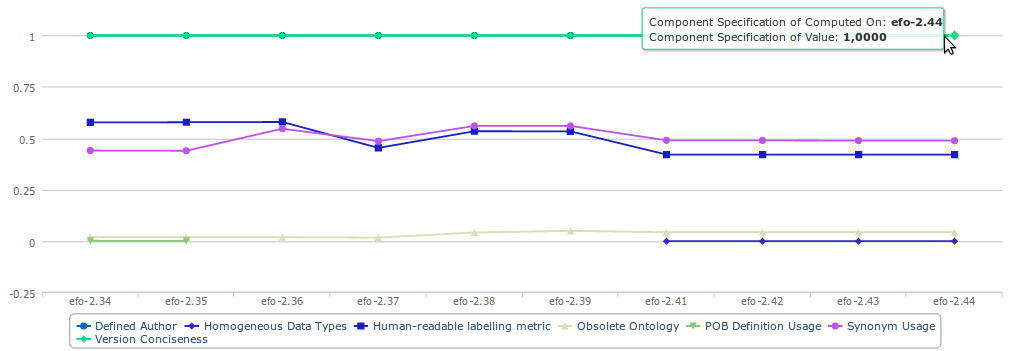
\includegraphics[scale=0.3]{images/cube_4.png} 
\caption{Lines Plot} 
\label{fig:line_chart}
\end{figure*}

A \emph{horizontal bar} represents each metric (Figure~\ref{fig:hor_chart}) and shows its value (x-axis) with respect to the dataset (y-axis).
Here, the different “datasets” analysed are actually successive revisions of one dataset.
This chart provides a clear view of how the value associated to each one of the measured metrics changes as the dataset evolves.
The horizontal layout is appropriate when the range of metric values is wide, and the number of different datasets is relatively small.

Similar to the horizontal bars chart, the \emph{vertical bar chart} (Figure~\ref{fig:ver_chart}) allows the user to compare the values computed for each of the metrics (y-axis), with respect to the dataset (x-axis).
In contrast with its horizontal counterpart, this chart is more appropriate when there are many datasets analysed but the range of metric values is not so wide.

In the \emph{radar chart} (Figure~\ref{fig:rad_chart}), the datasets are represented as slices of a circle and the values corresponding to the metrics are depicted as points and lines of a particular colour.
This chart provides a clear view of how the values of the metric differ from each other for each particular dataset. 
Furthermore, it allows one to assess the overall quality of a dataset, by showing whether the values of the metrics are concentrated around sections of the circle regarded as “good” or “bad”.

The lines plot (Figure~\ref{fig:line_chart}), lists the different datasets against the values of the metrics.
Here, where “different datasets” are actually different revisions in the evolution of one dataset, this plot provides a comparison of the evolution of the quality of the dataset, with respect to each metric.
The lines emphasise the points where the values of the metrics changed noticeably from one version to the next.


\subsubsection{Assessment Tab}
The Quality Framework Web-UI will also allow users to assess datasets for their quality.
Figure~\ref{fig:uiAssessementTab} shows a mockup of how the Assessment Tab will look like.
The user is guided step by step to assess a dataset:
\begin{enumerate}
\item The user choose the dataset to be assessed or give a dataset URI;
\item User decide what metrics to be assessed;
\item User decide if a quality problem report is required, which would allow the user to semi-automatically clean up the data (cf. Deliverable 3.1);
\item User clicks the \emph{assess} button to start assessing the chosen datasets.
\end{enumerate}

\begin{figure*}[tbph]
\center
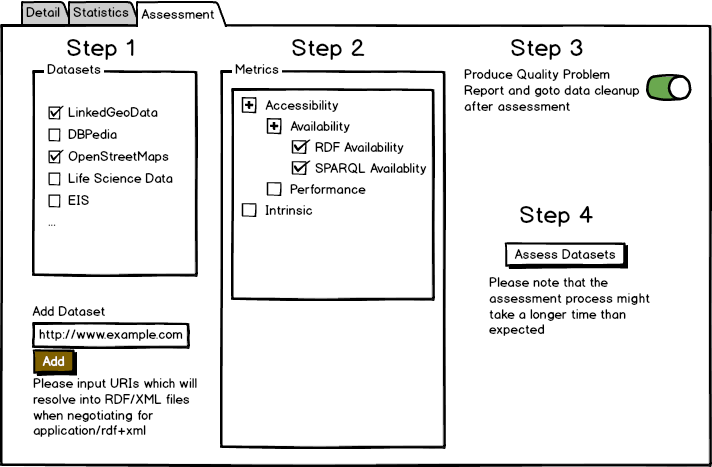
\includegraphics[width=\textwidth]{images/uiAssessmentTab.png} 
\caption{Mockup for the Assessment Tab} 
\label{fig:uiAssessementTab}
\end{figure*}

% describe the proposed UI mockups